\documentclass[pdflatex,sn-mathphys-num]{sn-jnl}% Math and Physical Sciences Numbered Reference Style

\usepackage{graphicx}%
\usepackage{multirow}%
\usepackage{amsmath,amssymb,amsfonts}%
\usepackage{amsthm}%
\usepackage{mathrsfs}%
\usepackage[title]{appendix}%
\usepackage{xcolor}%
\usepackage{textcomp}%
\usepackage{manyfoot}%
\usepackage{booktabs}%
\usepackage{algorithm}%
\usepackage{algorithmicx}%
\usepackage{algpseudocode}%
\usepackage{listings}%

\theoremstyle{thmstyleone}%
\newtheorem{theorem}{Theorem}%  meant for continuous numbers
\newtheorem{corollary}{Corollary}
\newtheorem{proposition}[theorem]{Proposition}% 
\theoremstyle{thmstyletwo}%
\newtheorem{example}{Example}%
\newtheorem{remark}{Remark}%
\theoremstyle{thmstylethree}%
\newtheorem{definition}{Definition}%
\raggedbottom

\begin{document}
\title[
A Projection Filtering Method for Output Redundant Systems
]{
A Projection Filtering Method for Output Redundant Systems
}


\author[1]{\fnm{Mehmet} \sur{Canevi}}\email{mehmet.canevi@ohu.edu.tr}
\author[2]{\fnm{Seyit Okan} \sur{Kara}}%\email{mehmet.canevi@ohu.edu.tr}

\affil*[1]{\orgdiv{Electrical-Electronics Engineering Department}, \orgname{Nigde Omer Halisdemir University}, \orgaddress{ \city{Nigde}, \postcode{51240}, \country{Turkey}}}
\affil[2]{\orgdiv{Bor Vocational School}, \orgname{Nigde Omer Halisdemir University}, \orgaddress{\city{Nigde}, \postcode{51240},\country{Turkey}}}


\abstract{

    We present a Projection Filtering Method(PFM) based on the gauge-invariance principle of modern physics, applicable to Output Redundant systems. A projection is proposed to use the invariance principle to decompose a linear output map into its components. In this work it is shown that, PFM can reconstruct states during the transient and steady state regime of dynamical systems and can serve as an alternative to classical observers for output redundant systems. Additionally, with PFM the reconstruction of states also translates into the reconstruction of disturbance, without the dependency on additional assumptions or a model of the disturbance, even with noisy outputs. The PFM is an alternative to classical observers for output redundant systems in this regard.

}

\keywords{projection, gauge-invariance, dynamical systems, observer, linear mapping, filter}

\maketitle

\section{INTRODUCTION}

Gauge invariance is a central organizing principle of modern physics, expressing the idea that observable quantities should remain unchanged under certain local transformations of the mathematical description. In classical field theories and quantum electrodynamics, this concept ensures that different representations related by gauge transformations correspond to the same physical reality~\cite{Peskin1995,YangMills1954}. From an abstract viewpoint, gauge invariance provides a systematic way to separate physically meaningful dynamics from redundant coordinate or potential offsets. This symmetry-based perspective has proven essential for constructing robust and consistent models in physics, and it motivates the extension of invariance principles beyond their traditional domain toward engineered dynamical systems subject to measurement distortions and unknown offsets.

In linear control systems, similar representation issues arise in the presence of redundant measurements or sensing architectures with non-minimal output representations. In particular, when the output matrix does not have full row rank, multiple output vectors may correspond to the same underlying state. This situation naturally appears in multi-sensor configurations, distributed systems, and sparse measurement settings, where the dimension of the measurement space exceeds the effective information content~\cite{Chen1999,Kailath1980}. As a result, the output representation contains directions that do not contribute to state observability but nevertheless affect the estimation process.

From this perspective, the measurement space can be decomposed into physically meaningful components and redundant directions that do not affect the underlying state. However, conventional observer designs typically treat all output components uniformly, without explicitly distinguishing between these subspaces. This may lead to estimation dynamics that are influenced by representation-dependent artifacts, rather than purely by physically relevant discrepancies.

This observation suggests that the estimation process should be constructed in a way that isolates the physically relevant part of the output from its redundant representation. A natural mechanism to achieve this separation is through a projection operator acting on the measurement space, which removes components lying in the non-informative directions while preserving the observable content. Such projection-based constructions are also well known in physics, particularly in gauge theories, where physically equivalent configurations are related by symmetry transformations and a representative is selected via gauge fixing~\cite{Peskin1995}.


In this work, we propose a way of constructing a projection that acts as a static filter to recover the linear output mapping in terms of its components under given constraints. This projection is given as an alternative to the classical observer design for output redundant systems, due to the fact that no dynamical estimation is necessary to reconstruct states and disturbances. 

The paper is organized as follows; preliminaries are given in section 2, the proposed projection filtering method is addressed in section 3. The proposed method is exemplified in section 4 with numerical examples. The conclusion and future work is given in section 5.

%%%%%%%%%%%%%%%%%%%%%%%%%%%%%%%%%%%%%%%%%%%%%%%%%%%%%%%%%%%%%%%%%%%%%%%%%%%%%%%%%%%%%%%%%%%%%%%%%%%%%%%%%%%%%%%%%%%%%%%%%%%%%%%%%%%%
\section{Preliminaries}
%%%%%%%%%%%%%%%%%%%%%%%%%%%%%%%%%%%%%%%%%%%%%%%%%%%%%%%%%%%%%%%%%
\subsection{The System Model}
%%%%%%%%%%%%%%%%%%%%%%%%%%%%%%%%%%%%%%%%%%%%%%%%%%%%%%%%%%%%%%%%%
Multi output linear time invariant dynamical systems are expressed as,
\begin{gather} 
    \dot{x}=A x+B_w w,\,y=C x+D_w w\label{eqn:lti1}
\end{gather}
where $x\in\mathbb{R}^{n\times 1}$ represents the state, $w\in\mathbb{R}^{r\times 1}$ originally the bias or more generally the exogenous input and $y\in\mathbb{R}^{p\times 1}$ is the measured output. The system matrices are defined as $A\in\mathbb{R}^{n\times n}$, $B_w\in\mathbb{R}^{n\times r}$, $C\in\mathbb{R}^{p\times n}$ and $D_w\in\mathbb{R}^{p\times r}$. Output redundant systems, which is a subset of dynamical control systems given in (\ref{eqn:lti1}), satisfy the following rank condition
\begin{gather}
    \mathrm{rank}(C)<p\label{eqn:rank_cond_sor}
\end{gather}
and arise in sparse sensor applications\cite{shoukry2015event}, topologies used in Multi Agent Systems(MAS)\cite{olfati2007consensus} and distributed networks \cite{yang2022sensor}. These systems are named Strictly Output Redundant(SOR) system according to \cite{yang2025output}. 
%%%%%%%%%%%%%%%%%%%%%%%%%%%%%%%%%%%%%%%%%%%%%%%%%%%%%%%%%%%%%%%%%
\subsection{The Luenberger Observer}
%%%%%%%%%%%%%%%%%%%%%%%%%%%%%%%%%%%%%%%%%%%%%%%%%%%%%%%%%%%%%%%%%
The Luenberger Observer is defined as,    
\begin{gather} 
    \dot{\hat{x}}=A \hat{x}+L(y-\hat{y}),\,\hat{y}=C \hat{x}
\end{gather}
where $L\in\mathbb{R}^{n\times p}$ is the observer gain. Assuming $(A,C)$-pair observable, the error dynamics are obtained for the error $e\triangleq x-\hat{x}$ as,
\begin{gather} 
    \dot{e}=(A-LC)e+(B_w-L D_w)w
\end{gather}
The mixed $\mathcal{H}_2/\mathcal{H}_\infty$ optimal observer for objective function $z=C_ze$ is designed using the following LMI problem\cite{duan2013lmis},
\begin{equation} \label{eqn:lmi1}
\begin{split} 
    \min_{Z,Y,P}{(\gamma_\infty+\gamma_2)}\quad \mathrm{s.t.}\\
    \begin{bmatrix}
        (PA-YC)+(\star)^T& PB_w-YD_w& C_z^T\\
        \star& -\gamma_\infty I& 0\\
        \star& 0& -\gamma_\infty I
    \end{bmatrix}\prec 0\\
    \mathrm{trace}(Z)\leq \gamma_2\\
    \begin{bmatrix}
       P& \star\\
       C_z& Z
    \end{bmatrix}\succ 0\\
    P\succ 0
\end{split} 
\end{equation}
where the observer gain is recovered with $L=P^{-1}Y$ and the problem can be solved using convex programs \cite{cvx},\cite{gb08}. 

In addition to classical observers, unknown input observer (UIO) frameworks have been developed to decouple disturbances from state estimation \cite{ChenPatton1999}.

\subsection{Miscellaneous}
The null space of a matrix $X$ is denoted by $\mathcal{N}(X)$ where the columns space of $X$ is denoted by $\mathcal{R}(X)$. 
The Moore-Penrose pseudo-inverse is denoted with $(.)^\dagger$ and for full row-rank matrix $X$ is defined as,
\begin{equation}
    X^\dagger=X^T(XX^T)^{-1}
\end{equation}
%%%%%%%%%%%%%%%%%%%%%%%%%%%%%%%%%%%%%%%%%%%%%%%%%%%%%%%%%%%%%%%%%
\section{Projection Filtering}
%%%%%%%%%%%%%%%%%%%%%%%%%%%%%%%%%%%%%%%%%%%%%%%%%%%%%%%%%%%%%%%%%
In any linear dynamical system with linear output mapping where output redundancy is present, the structure can be exploited to separate the output into its components. By using Gauge-Invariance principle a projection operator can be chosen to truncate some of the subcomponents of the output mapping to isolate the component under interest. 

The idea of separating disturbance and state components is closely related to disturbance decoupling problems studied in geometric control theory \cite{BasileMarro1992}.

%%%%%%%%%%%%%%%%%%%%%%%%%%%%%%%%%%%%%%%%%%%%%%%%%%%%%%%%%%%%%%%%%
\begin{theorem}%[Orthogonal Complement Projection]
Let $X\in \mathbb{R}^{s\times n}$ be a matrix with $\mathrm{rank}(X)=n\leq s$. There exists a unique projection matrix $\Pi^X\in\mathbb{R}^{s\times s}$ that is defined by:
\begin{equation*}
    \Pi^X\triangleq I_s-X{(X^T X)}^{-1}X^T \label{eq:projection}
\end{equation*}
satisfying the following properties:
\begin{itemize}
    \item (\textit{Annihilation}) $\Pi^X X=0$.
    \item (\textit{Invariance}) $\Pi^X z=z,\,\forall z\in\mathcal{N}(X^T)$.
    \item (\textit{Existence}) $\Pi^X \neq 0 \iff \mathrm{rank}(X)<s$.
\end{itemize}
\end{theorem}
    \begin{proof}
        \begin{itemize}
        \item (\textit{Annihilation}) 
        Plugging in the definition of $\Pi^X$ gives,
        \begin{equation*}
        \begin{split}
            \Pi^X X&=(I_s-X{(X^T X)}^{-1}X^T) X\\
            &=X-X{(X^T X)}^{-1}{(X^T X)}=0
        \end{split}
        \end{equation*}
        \item (\textit{Invariance})
        By definition of $z\in\mathcal{N}(X^T)$, utilizing $X^T z=0$ and plugging in the definition of $\Pi^X$ gives,
        \begin{equation*}
        \begin{split}
            \Pi^X z&=(I_s-X{(X^T X)}^{-1}X^T) z\\
            &=z-X{(X^T X)}^{-1}X^T z=z
        \end{split}
        \end{equation*}
        \item (\textit{Existence})
        Let $\Pi^X\neq 0$, by definition 
        \begin{equation*}
        \begin{split}
            \Pi^X &=I_s-X{(X^T X)}^{-1}X^T \\
            &=I_s-X{(X^T X)}^{-1}X^T\neq 0
        \end{split}
        \end{equation*}
        then $I_s\neq X{(X^T X)}^{-1}X^T$ and 
        \begin{equation*}
        \begin{split}
            \mathrm{rank}(\Pi^X) &\geq 1 \\
            \mathrm{rank}(I_s)-\mathrm{rank}(X{(X^T X)}^{-1}X^T)&\geq 1 \\
            s-\mathrm{rank}(X)&\geq 1\\
            s&\geq \mathrm{rank}(X)+1\\
            \mathrm{rank}(X)&<s
        \end{split}
        \end{equation*}
        Let $\mathrm{rank}(X)<s$, $\exists v\neq 0\in\mathcal{N}(X^T)$, then, $X^T v=0$ and
        \begin{equation*}
            \Pi^X v=(I_s-X{(X^T X)}^{-1}X^T)v=v-0=v
        \end{equation*}
        Since $\Pi^X v=v$ and $v\neq 0$, $\Pi^X v\neq 0$, hence $\Pi^X\neq 0$.
    \end{itemize}
\end{proof}


\begin{corollary}[Invariance and Recovery]
For the measurement equation $y = Cx + D_w w$ and under assumptions $\mathrm{rank}(C) < p$ and $\mathrm{rank}(D_w) < p$, the following invariance and recovery properties hold:
\begin{itemize}
    \item (\textit{State Invariance}) $\Pi^C y$ isolates the state invariant part $\Pi^C D_w w$ of the measurement equation. 
    \item (\textit{Disturbance invariance}) $\Pi^{D_w}$ isolates the disturbance invariant part $\Pi^{D_w} C x$ of the measurement equation.
    \item (\textit{Recoverability}) The disturbance $w$ is recoverable via $\hat{w} = (\Pi^C D_w)^\dagger \Pi^C y$ and the state $x$ is recoverable via $\hat{x} = (\Pi^{D_w}C)^\dagger \Pi^{D_w} y$ if and only if $\mathcal{R}(D_w) \not\subseteq \mathcal{R}(C)$.
\end{itemize}
\end{corollary}

\begin{proof}
    Applying $\Pi^C$ to the output yields $\Pi^C y = \Pi^C Cx + \Pi^C D_w w$. From the \textit{Annihilation} property of Theorem 1, $\Pi^C C = 0$, which proves (\textit{State Invariance}). 
    
    Similarly, for (\textit{Disturbance invariance}), $\Pi^{D_w} (Cx + D_w w)=\Pi^{D_w} Cx$.
    
    The condition $\mathcal{R}(D_w) \not\subseteq \mathcal{R}(C)$ ensures both $\Pi^C D_w \neq 0$ and $\Pi^{D_w}C\neq 0$, the terms $\Pi^C D_w$ and $\Pi^{D_w} C$ remain, which proves (\textit{Recoverability}).
\end{proof}


%%%%%%%%%%%%%%%%%%%%%%%%%%%%%%%%%%%%%%%%
The projection filtering method (PFM) is based on the projection matrix defined in Theorem~1 where both the states and the disturbance of (\ref{eqn:lti1}) can be isolated and thereby invariance to each component can be achieved. The states and the disturbance are recovered using Corollary~1.1 (\textit{Recoverability}). Theorem~1 (\textit{Existence}) is aligned with the output redundancy of (\ref{eqn:lti1}). Assuming Corollary~1.1 (\textit{Recoverability}) holds, the least square estimator for disturbance is given as,
\begin{gather}
    \hat{w}=(\Pi^C D_w)^\dagger(\Pi^C y)\label{eqn:filtering_w}
\end{gather}
where for the states the estimator is given as
\begin{gather}
    \hat{x}=(\Pi^{D_w}C)^\dagger(\Pi^{D_w} y)\label{eqn:filtering_x}
\end{gather}

%%%%%%%%%%%%%%%%%%%%%%%%%%%%%%%%%%%%%%%%
\begin{corollary}[Generalization]
Consider a sum of $k$ signals defined as follows,
\begin{equation*}
    y = \sum_{i=1}^k M_i \xi_i
\end{equation*}
where $M_i \in \mathbb{R}^{s \times n_i}$. Any specific component $\xi_j$ can be isolated from all other components $\{ \xi_i \}_{i \neq j}$ by applying the projection $\Pi^{\bar{M}_j}$, where $\bar{M}_j = [M_1, \dots, M_{j-1}, M_{j+1}, \dots, M_k]$. Applying the projection to $y$ yields,
\begin{equation*}
    \Pi^{\bar{M}_j} y = \Pi^{\bar{M}_j} M_j \xi_j
\end{equation*}
Furthermore, $\xi_j$ is recoverable if and only if $\mathrm{rank}([\bar{M}_j, M_j]) > \mathrm{rank}(\bar{M}_j)$, which is satisfied if $\mathcal{R}(M_j) \not\subseteq \mathcal{R}(\bar{M}_j)$.
\end{corollary}

\begin{proof}
The proof follows directly from the \textit{Annihilation} property of Theorem 1. By defining the augmented matrix $\bar{M}_j$, the projection $\Pi^{\bar{M}_j}$ satisfies $\Pi^{\bar{M}_j} \bar{M}_j = 0$. Since $\bar{M}_j$ contains all matrices $M_i$ except $M_j$, all terms $M_i \xi_i$ for $i \neq j$ vanish, leaving only the $j$-th component.
\end{proof}

Corollary~1.2 is given to illustrate that PFM can be applied to generalized linear output maps, especially to measurement equations in the following manner,
\begin{equation} 
    y=Cx+D_w w+D_n n
\end{equation} 
As addressed in the next section, PFM can be applied to noisy measurement equations. 

Both the state and disturbance signals are reconstructed rather than being estimated, exploiting the structural advantage of the output redundancy of systems defined with (\ref{eqn:lti1}). As it is illustrated in the next section, using PFM, the measured output is decomposed into its state and disturbance components algebraically, which shows that the projection filtering eliminates the requirement of individual observers to estimate the states and disturbances of such systems. PFM is also applicable to outputs with noise.


%%%%%%%%%%%%%%%%%%%%%%%%%%%%%%%%%%%%%%%%%%%%%%%%%%%%%%%%%%%%%%%%%%%%%%%%%%%%%%%%%%%%%%%%%%%%%%%%%%%%%%%%%%%%%%
\section{Numerical Examples}
A comparison between the dynamic state estimation of a Luenberger observer and the algebraic recovery of both state and disturbance of the projection filtering method is given in Example 1. Noise is added in Example 2, in order to showcase that the projection filtering method is able to handle noise in measurements, by the cost of an additional sensor. 
\subsection{Example 1}
The electrical system given in\cite{yang2025output} with parameters $C_t=2.2\mathrm{mF}$, $L_t=1.8\mathrm{mH}$ and $R_t=0.2\Omega$ is defined as the following state space model,
\begin{equation}
A=\begin{bmatrix}
    0& \frac{1}{C_t}\\
    -\frac{1}{L_t}& -\frac{-R_t}{L_t}    
\end{bmatrix},\,
B_w=\begin{bmatrix}
    -\frac{1}{C_t}\\
    0    
\end{bmatrix},\,
C=\begin{bmatrix}
    1& 0\\    
    1& 0\\    
    0& 1    
\end{bmatrix}
\end{equation}
where output redundancy is created by replicating the sensor measuring first state. The exogenous input matrix is constructed as follows,
\begin{equation}
    D_w=C^\perp+C\begin{bmatrix}1\\1\end{bmatrix}=\begin{bmatrix}
    1.7071\\
    0.2929\\
    1.0000
    \end{bmatrix}
\end{equation}
A Luenberger observer is designed solving the LMI given in (\ref{eqn:lmi1}) assuming $C_z=I$. Solving the corresponding LMI, yields,
\begin{equation}
    Y=\begin{bmatrix}
 -159314.9& 7541099.0& -12347840.0\\
-1741760.0& 3556493.0&   3485615.0
    \end{bmatrix}
\end{equation}
and
\begin{equation}
    Z=\begin{bmatrix}
    0.0000449847& 0.00000887586\\
    0.00000887586&  0.0000594674
    \end{bmatrix}
\end{equation}
with $\gamma_\infty=0.0012$, $\gamma_2=0.0001044$. The observer gain and Lyapunov matrix are determined as,
\begin{equation}
    L=\begin{bmatrix}
    -22.6263&  370.8001& -524.5247\\
    -104.9918&  278.4287&   97.6824
    \end{bmatrix}
\end{equation}
and 
\begin{equation}
    P=\begin{bmatrix}
    22904.36& -3418.62\\
    -3418.62&  17326.22
    \end{bmatrix}
\end{equation}
noting that $B_w-LD_w=0$ is satisfied, hence the state estimation is not affected by the exogenous input. No assumption about the exogenous input is added, thus the estimated state is utilized to obtain the exogenous input with,
\begin{equation}
    \hat{w}=D_w^\dagger(y-Cx)
\end{equation}

On the other hand, using PFM the projection matrix given by Theorem~1 is determined for $C$ as,
\begin{equation}
\Pi^C=\begin{bmatrix}
    0.5&   -0.5&         0\\
    -0.5&    0.5&         0\\
    0&        0&         0
\end{bmatrix}
\end{equation}
and for $D_w$ as,
\begin{equation}
\Pi^{D_w}=\begin{bmatrix}
    0.2714&   -0.1250&   -0.4268\\
   -0.1250&    0.9786&   -0.0732\\
   -0.4268&   -0.0732&    0.7500\\
\end{bmatrix}
\end{equation}
The disturbance and the states are filtered using (\ref{eqn:filtering_w}) and (\ref{eqn:filtering_x}), respectively.
The state estimation and the projection state filtering is compared in Figure~\ref{fig:ex1_states1}.
\begin{figure}[!htb]
    \centering
    
\includegraphics[width=0.85\linewidth]{ex1_states1}
    \caption{Comparison of the Luenberger observer state estimation versus projection filtering state reconstruction.}
    \label{fig:ex1_states1}
\end{figure}

The estimation process of the Luenberger observer takes $0.01$ seconds due to the fact that the observer is a dynamic observer, whereas the projection filtering directly matches the original system states at $t=0$ seconds as illustrated in Figure~\ref{fig:ex1_states1}. It is possible to decrease the estimation duration of the observer by speeding up the observer eigenvalues, but in return the observer gain and therefore noise amplification would increase. 


% The exogenous input estimated and filtered is depicted in Figure~\ref{fig:ex1_disturbance}.
\begin{figure}[!htb]
    \centering
    
\includegraphics[width=0.85\linewidth]{ex1_disturbance}
    \caption{Estimated disturbance using Luenberger Observer versus reconstructed disturbance of the projection filtering}
    \label{fig:ex1_disturbance}
\end{figure}

The Luenberger observer is a state estimator, but using the linear mapping of the output, it is possible to reconstruct the disturbance assuming the lack of noise in the measured output. It also possible to employ a Disturbance Observer, but then it is necessary to also assume a certain model or add an assumption about the disturbance. This extra information about the disturbance is not necessary for the projection filtering method. 
As illustrated in Figure~\ref{fig:ex1_disturbance}, the reconstruction of the disturbance using the Luenberger observer state matches the disturbance only in the steady state, since the state estimation gets corrected during the transients. But, the projection filtering method results in an exact match, due to its static approach.


% The projection filtering method utilizes the geometric properties of the output mapping, hence no dynamic estimation is present, it directly extracts the output map into its components. Despite the fact that the Luenberger observer gain for output redundant systems is able to eliminate the exogenous input term in the error dynamic by setting $B_w-LD_w$ to zero, the structure exploit performs better for the given example since no estimation takes place. Static output filtering fails if 
% \begin{equation}
%     D_w=C\alpha
% \end{equation}
% since,
% \begin{equation}
%     \Pi y=\Pi Cx+\Pi D_w w=\Pi C(x+\alpha)=0
% \end{equation}
% which shows that different channels need to exist in order separate signals using the projection. 

\subsection{Example 2}
In most practical applications noise is present in measured outputs as given in,
\begin{equation}
    y=Cx+D_w w+D_n n\label{eqn:ex2_output_mapping1}
\end{equation}
For illustrative purposes the following output equation is defined
\begin{equation}
    y=\begin{bmatrix}
    1&     0\\
    2&     1\\
    0&     1\\
    0&     1
    \end{bmatrix}x(t)+\begin{bmatrix}
        2.2060\\
        2.3970\\
        1.3015\\
        1.3015
    \end{bmatrix}w(t)+
    \begin{bmatrix}
    0.1960\\
    0.7382\\
    0.6697\\
    0.5265
    \end{bmatrix}n(t)
\end{equation}
where $w(t)$ is disturbance, $n(t)$ is noise and $x(t)$, which represent some system states and  are arbitrarily chosen as,
\begin{equation}
    x(t)=\begin{bmatrix}
        \sin(t)\\ \cos(t)
    \end{bmatrix}
\end{equation}
In order to be able to recover both the states and the disturbance in such a system, the number of sensors for measurement needs to increase, since the amount of total unknown signals in (\ref{eqn:ex2_output_mapping1}) requires equal amount of measurements. Otherwise, the least square estimation will be the only recovery attainable. 

The disturbance matrix is defined using 
\begin{equation}
    D_w=C\begin{bmatrix}1\\1\end{bmatrix}+C^\perp\begin{bmatrix}1\\1\end{bmatrix}
\end{equation}
and the noise matrix $D_n$ is chosen as a random matrix.

The output mapping in (\ref{eqn:ex2_output_mapping1}) is rewritten as,
\begin{equation}
    y=Cx+\begin{bmatrix}
        D_w& D_n
    \end{bmatrix}\begin{bmatrix}
    w\\n        
    \end{bmatrix}
\end{equation}
and the projection defined using Corollary~1.2 to recover the state information $x(t)$ can be calculated using,
\begin{equation}
    \Pi^{wn}=I-\begin{bmatrix}
        D_w& D_n
    \end{bmatrix}\left(
        \begin{bmatrix}
        D_w\\ D_n
    \end{bmatrix}\begin{bmatrix}
        D_w& D_n
    \end{bmatrix}
    \right)^{-1}\begin{bmatrix}
        D_w\\D_n
    \end{bmatrix}
\end{equation}
and is determined as
\begin{equation}
    \Pi^{wn}=\begin{bmatrix}
    0.6224&   -0.2581&   -0.3034&   -0.2763\\
    -0.2581&    0.1118&    0.1698&    0.0618\\
    -0.3034&    0.1698&    0.5564&   -0.3549\\
    -0.2763&    0.0618&   -0.3549&    0.7094
    \end{bmatrix}
\end{equation}
Then the state $x(t)$ is recovered using,
\begin{equation}
    \hat{x}=(\Pi^{wn}C)^\dagger (\Pi^{wn}y)
\end{equation}

\begin{figure}[!htb]
    \centering
    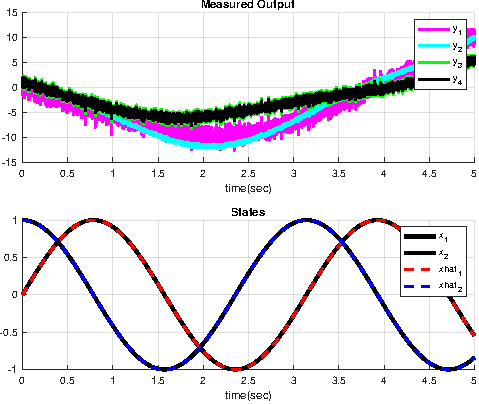
\includegraphics[width=0.85\linewidth]{ex2_results}
    \caption{The measured outputs($y_1$, $y_2$, $y_3$, $y_4$) and the states($x_1$, $x_2$) versus the projection filtering method recovered states($\hat{x}_1$, $\hat{x}_2$)}
    \label{fig:ex2_results}
\end{figure}
The measured output for each sensor with noise is depicted in Figure~\ref{fig:ex2_results}. The output redundancy can be observed by comparing third output and fourth output in Figure~\ref{fig:ex2_results}. It can also be seen that the projection filtering method is able to reconstruct both states under noisy measurements.

\begin{figure}[!htb]
    \centering
    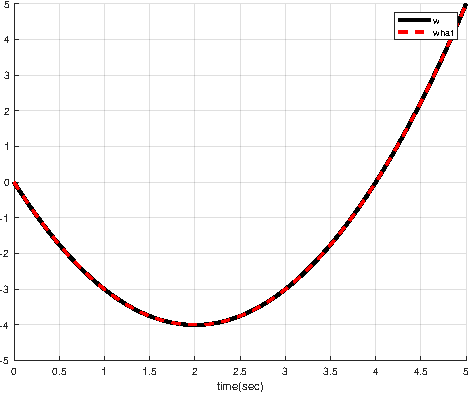
\includegraphics[width=0.85\linewidth]{ex2_results2}
    \caption{Disturbance recovered by projection filtering versus actual disturbance}
    \label{fig:ex2_results2}
\end{figure}


The disturbance is recovered using the projection on $\begin{bmatrix}
        C& D_n
    \end{bmatrix}$ as,
\begin{gather}
    \Pi^{xn}=\begin{bmatrix}
     0.7254&   -0.3627&    0.1507&    0.2120\\
   -0.3627 &   0.1813 &  -0.0754 &  -0.1060\\
    0.1507 &  -0.0754 &   0.0313 &   0.0440\\
    0.2120 &  -0.1060 &   0.0440 &   0.0619
    \end{bmatrix}
\end{gather}
and is plotted in Figure~\ref{fig:ex2_results2}. It is observed that disturbance recovery works in a similar fashion compared to state recovery in Figure~\ref{fig:ex2_results}. 


Throughout the examples given in this section, it has been established that, the projection filtering method exploits the output mapping using a projection matrix and recovers the states and the disturbance of a system directly. Whereas, the Luenberger observer, however fast dynamics it possesses, estimates the states of a system, due to its dynamic structure. Assuming no information about disturbance, one can also back-calculate the disturbance in a system with the Luenberger state estimates. Due to the dynamics, the disturbance and state estimations are valid for steady-state. But projection filtering gives valid results for both transient and steady-state regime. Additionally, projection filtering can handle noise, if necessary amount of sensors are present. 


\section{Conclusion and Future Work}

For estimation of states of output redundant systems, the Luenberger observer is a classical tool. This extends to disturbance estimation, if a model or additional assumptions are made for the disturbance. 

However, it has been shown that, for output redundant systems, a projection filtering method can be used to both reconstruct the states and disturbances. The PFM is based on the gauge-invariance principle, where the invariance can be chosen to isolate components for recovery under appropriate transformations, which then in turn is used to separate the linear mapping in the output. It has been noted that the separation is a static process, rather than an estimation process. It has been observed that, the static nature proves to be an important advantage, since this can be achieved with high gain Luenberger observers, but with a cost of higher noise amplification. 

It is also shown that, the PFM can be applied for outputs where noise is present. It is observed that the PFM is an alternative to classical observers for output redundant systems.

A natural extension of this work is to apply PFM to systems with nonlinear dynamics and output mappings, etc. 

%% Declarations
\section*{DECLARATIONS}
 
\subsection*{Conflict of Interest}
The authors declare that there is no competing financial interest or personal relationship that could have appeared to influence the work reported in this paper.
 
\subsection*{Authors’ Contributions}
Seyit Okan Kara contributed to conceptualization, writing, methodology and Mehmet Canevi contributed to conceptualization, writing, methodology and software.
 
\subsection*{Funding}
Not Applicable.
 
\subsection*{Data Availability}
The data that support the findings of this study are
available from the corresponding author upon reasonable request.

% \bibliography{sn-bibliography}% common bib file
% %% if required, the content of .bbl file can be included here once bbl is generated
% %%\input sn-article.bbl

% \bibliography{library}    


\begin{thebibliography}{13}
% BibTex style file: bmc-mathphys.bst (version 2.1), 2014-07-24
\ifx \bisbn   \undefined \def \bisbn  #1{ISBN #1}\fi
\ifx \binits  \undefined \def \binits#1{#1}\fi
\ifx \bauthor  \undefined \def \bauthor#1{#1}\fi
\ifx \batitle  \undefined \def \batitle#1{#1}\fi
\ifx \bjtitle  \undefined \def \bjtitle#1{#1}\fi
\ifx \bvolume  \undefined \def \bvolume#1{\textbf{#1}}\fi
\ifx \byear  \undefined \def \byear#1{#1}\fi
\ifx \bissue  \undefined \def \bissue#1{#1}\fi
\ifx \bfpage  \undefined \def \bfpage#1{#1}\fi
\ifx \blpage  \undefined \def \blpage #1{#1}\fi
\ifx \burl  \undefined \def \burl#1{\textsf{#1}}\fi
\ifx \doiurl  \undefined \def \doiurl#1{\url{https://doi.org/#1}}\fi
\ifx \betal  \undefined \def \betal{\textit{et al.}}\fi
\ifx \binstitute  \undefined \def \binstitute#1{#1}\fi
\ifx \binstitutionaled  \undefined \def \binstitutionaled#1{#1}\fi
\ifx \bctitle  \undefined \def \bctitle#1{#1}\fi
\ifx \beditor  \undefined \def \beditor#1{#1}\fi
\ifx \bpublisher  \undefined \def \bpublisher#1{#1}\fi
\ifx \bbtitle  \undefined \def \bbtitle#1{#1}\fi
\ifx \bedition  \undefined \def \bedition#1{#1}\fi
\ifx \bseriesno  \undefined \def \bseriesno#1{#1}\fi
\ifx \blocation  \undefined \def \blocation#1{#1}\fi
\ifx \bsertitle  \undefined \def \bsertitle#1{#1}\fi
\ifx \bsnm \undefined \def \bsnm#1{#1}\fi
\ifx \bsuffix \undefined \def \bsuffix#1{#1}\fi
\ifx \bparticle \undefined \def \bparticle#1{#1}\fi
\ifx \barticle \undefined \def \barticle#1{#1}\fi
\bibcommenthead
\ifx \bconfdate \undefined \def \bconfdate #1{#1}\fi
\ifx \botherref \undefined \def \botherref #1{#1}\fi
\ifx \url \undefined \def \url#1{\textsf{#1}}\fi
\ifx \bchapter \undefined \def \bchapter#1{#1}\fi
\ifx \bbook \undefined \def \bbook#1{#1}\fi
\ifx \bcomment \undefined \def \bcomment#1{#1}\fi
\ifx \oauthor \undefined \def \oauthor#1{#1}\fi
\ifx \citeauthoryear \undefined \def \citeauthoryear#1{#1}\fi
\ifx \endbibitem  \undefined \def \endbibitem {}\fi
\ifx \bconflocation  \undefined \def \bconflocation#1{#1}\fi
\ifx \arxivurl  \undefined \def \arxivurl#1{\textsf{#1}}\fi
\csname PreBibitemsHook\endcsname

%%% 1
\bibitem[\protect\citeauthoryear{Peskin and Schroeder}{1995}]{Peskin1995}
\begin{bbook}
\bauthor{\bsnm{Peskin}, \binits{M.E.}},
\bauthor{\bsnm{Schroeder}, \binits{D.V.}}:
\bbtitle{An Introduction to Quantum Field Theory}.
\bpublisher{Addison-Wesley},
(\byear{1995})
\end{bbook}
\endbibitem

%%% 2
\bibitem[\protect\citeauthoryear{Yang and Mills}{1954}]{YangMills1954}
\begin{barticle}
\bauthor{\bsnm{Yang}, \binits{C.N.}},
\bauthor{\bsnm{Mills}, \binits{R.L.}}:
\batitle{Conservation of isotopic spin and isotopic gauge invariance}.
\bjtitle{Phys. Rev.}
\bvolume{96},
\bfpage{191}--\blpage{195}
(\byear{1954})
\end{barticle}
\endbibitem

%%% 3
\bibitem[\protect\citeauthoryear{Chen}{1999}]{Chen1999}
\begin{bbook}
\bauthor{\bsnm{Chen}, \binits{C.-T.}}:
\bbtitle{Linear System Theory and Design}.
\bpublisher{Oxford University Press}, 
(\byear{1999})
\end{bbook}
\endbibitem

%%% 4
\bibitem[\protect\citeauthoryear{Kailath}{1980}]{Kailath1980}
\begin{bbook}
\bauthor{\bsnm{Kailath}, \binits{T.}}:
\bbtitle{Linear Systems}.
\bpublisher{Prentice-Hall}, 
(\byear{1980})
\end{bbook}
\endbibitem

%%% 5
\bibitem[\protect\citeauthoryear{Shoukry and Tabuada}{2015}]{shoukry2015event}
\begin{barticle}
\bauthor{\bsnm{Shoukry}, \binits{Y.}},
\bauthor{\bsnm{Tabuada}, \binits{P.}}:
\batitle{Event-triggered state observers for sparse sensor noise/attacks}.
\bjtitle{IEEE Transactions on Automatic Control}
\bvolume{61}(\bissue{8}),
\bfpage{2079}--\blpage{2091}
(\byear{2015})
\end{barticle}
\endbibitem

%%% 6
\bibitem[\protect\citeauthoryear{Olfati-Saber
  et~al.}{2007}]{olfati2007consensus}
\begin{barticle}
\bauthor{\bsnm{Olfati-Saber}, \binits{R.}},
\bauthor{\bsnm{Fax}, \binits{J.A.}},
\bauthor{\bsnm{Murray}, \binits{R.M.}}:
\batitle{Consensus and cooperation in networked multi-agent systems}.
\bjtitle{Proceedings of the IEEE}
\bvolume{95}(\bissue{1}),
\bfpage{215}--\blpage{233}
(\byear{2007})
\end{barticle}
\endbibitem

%%% 7
\bibitem[\protect\citeauthoryear{Yang et~al.}{2022}]{yang2022sensor}
\begin{barticle}
\bauthor{\bsnm{Yang}, \binits{G.}},
\bauthor{\bsnm{Rezaee}, \binits{H.}},
\bauthor{\bsnm{Serrani}, \binits{A.}},
\bauthor{\bsnm{Parisini}, \binits{T.}}:
\batitle{Sensor fault-tolerant state estimation by networks of distributed
  observers}.
\bjtitle{IEEE Transactions on Automatic Control}
\bvolume{67}(\bissue{10}),
\bfpage{5348}--\blpage{5360}
(\byear{2022})
\end{barticle}
\endbibitem

%%% 8
\bibitem[\protect\citeauthoryear{Yang et~al.}{2025}]{yang2025output}
\begin{botherref}
\oauthor{\bsnm{Yang}, \binits{G.}},
\oauthor{\bsnm{Gallo}, \binits{A.J.}},
\oauthor{\bsnm{Barboni}, \binits{A.}},
\oauthor{\bsnm{Ferrari}, \binits{R.M.}},
\oauthor{\bsnm{Serrani}, \binits{A.}},
\oauthor{\bsnm{Parisini}, \binits{T.}}:
On the output redundancy of lti systems: A geometric approach with application
  to privacy.
IEEE Transactions on Automatic Control
(2025)
\end{botherref}
\endbibitem

%%% 9
\bibitem[\protect\citeauthoryear{Duan and Yu}{2013}]{duan2013lmis}
\begin{bbook}
\bauthor{\bsnm{Duan}, \binits{G.-R.}},
\bauthor{\bsnm{Yu}, \binits{H.-H.}}:
\bbtitle{LMIs in Control Systems: Analysis, Design and Applications}.
\bpublisher{CRC press}, 
(\byear{2013})
\end{bbook}
\endbibitem

%%% 10
\bibitem[\protect\citeauthoryear{Grant and Boyd}{2014}]{cvx}
\begin{botherref}
\oauthor{\bsnm{Grant}, \binits{M.}},
\oauthor{\bsnm{Boyd}, \binits{S.}}:
{CVX}: Matlab Software for Disciplined Convex Programming, version 2.1
(2014)
\end{botherref}
\endbibitem

%%% 11
\bibitem[\protect\citeauthoryear{Grant and Boyd}{2008}]{gb08}
\begin{bchapter}
\bauthor{\bsnm{Grant}, \binits{M.}},
\bauthor{\bsnm{Boyd}, \binits{S.}}:
\bctitle{Graph implementations for nonsmooth convex programs}.
In: \beditor{\bsnm{Blondel}, \binits{V.}},
\beditor{\bsnm{Boyd}, \binits{S.}},
\beditor{\bsnm{Kimura}, \binits{H.}} (eds.)
\bbtitle{Recent Advances in Learning and Control}.
\bsertitle{Lecture Notes in Control and Information Sciences},
pp. \bfpage{95}--\blpage{110}.
\bpublisher{Springer}, 
(\byear{2008})
\end{bchapter}
\endbibitem

%%% 12
\bibitem[\protect\citeauthoryear{Chen and Patton}{1999}]{ChenPatton1999}
\begin{bbook}
\bauthor{\bsnm{Chen}, \binits{J.}},
\bauthor{\bsnm{Patton}, \binits{R.J.}}:
\bbtitle{Robust Model-Based Fault Diagnosis for Dynamic Systems}.
\bpublisher{Kluwer Academic Publishers}, 
(\byear{1999})
\end{bbook}
\endbibitem

%%% 13
\bibitem[\protect\citeauthoryear{Basile and Marro}{1992}]{BasileMarro1992}
\begin{bbook}
\bauthor{\bsnm{Basile}, \binits{G.}},
\bauthor{\bsnm{Marro}, \binits{G.}}:
\bbtitle{Controlled and Conditioned Invariants in Linear System Theory}.
\bpublisher{Prentice Hall}, 
(\byear{1992})
\end{bbook}
\endbibitem

\end{thebibliography}


\end{document}
